\chapter{Entropy-based measures of verbal valency}\label{chapter:entropy}

While the previous chapter has demonstrated that corpus-based transitivity ratios can serve as a useful basis for typological comparison, it is still is a relatively simple metric that captures one aspect of verbal valency. Put another way, transitivity ratio can be seen as a subset of the scope needed for a more holistic investigation into verbal valency, as it concerns only one type of verb dependent, i.e., the object, and one feature of this dependent, i.e., its presence or absence. 

This chapter undertakes to expand the scope of investigation accordingly, to cover both more verb dependent types and more features of them. Instead of performing exhaustive comparisons on each individual feature of each dependent, the focus is on the variability of \textit{valency frame alternations} (also called diathesis alternations), i.e., the range of valency frames in which a verb appears and how likely it is to appear with each frame. New entropy-based measures of verbal valency are proposed and tested in conjunction with hypotheses about the structure of valency systems.

The sections are organized as follows: §\ref{sec:entropy-background} provides a brief background on cognitive and psycholinguistic perspectives on language structure, in particular relating to the frequency effect and valency frame alternation, which motivate the hypotheses tested in the experiments; in §\ref{sec:valency-frame-encoding}, the feature selection and extraction procedures of valency frame encoding from UD are described, as they form the basis for the experiments in this chapter. 

Four experiments are then presented: Experiment 2 (§\ref{sec:exp2-valency-frame-entropy}) uses joint entropy to define the valency frame entropy measure and tests its correlation with verb frequency; Experiment 3 (§\ref{sec:exp3-ablation}) examines cross-lingual variations in how languages encode the valency frames, by means of an ablation study using conditional entropy to assess the contribution of word order and case marking to the overall valency frame entropy; Experiment 4 (§\ref{sec:exp4-verb-specificity}) uses conditional entropy measure and seeks to quantitatively verify the verb specificity test that is used to distinguish core and non-core dependents (complements and adjuncts); Experiment 5 (§\ref{sec:exp5-verb-entropy}) takes a frame-based approach and, in symmetry to Experiment 2, calculates the correlation between verb entropy and frame frequency.

\section{Valency frame, frequency and the efficient organization of the lexicon}\label{sec:entropy-background}

Cognitive linguists and typologists have increasingly sought to integrate the two approaches in the same functionalist research paradigm \citep{croft2016}. Among others is research that seeks to examine and explain language-internal and cross-linguistic features of human languages through the lens of communicative efficiency, at various levels including the lexicon, syntax and morphology (see \citealp{gibson2019} for a survey). 

An early example where efficiency is used to explain phenomena in human languages is the work of George Kingsley \citet{zipf1935,zipf1949}. He first studied what is now known as Zipf's law, the empirical observation of the negative correlation between word length and frequency, that ``the magnitude of words tends, on the whole, [stands] in an inverse (not necessarily proportionate) relationship to the number of occurrences'', and sought to explain it through the principle of least effort.

Frequency is a particularly frequent lens through which the lexicon is examined and the correlation between frequency and other features often subjects of hypotheses. Its importance has been further underlined by psycholinguistic studies which show a consistent ``frequency effect'' for both open and closed class word \citep{segui1982,marslen-wilson1990}, where more frequently occurring words have a higher resting activation, making their lexical retrieval easier. That the most frequent lexical items are also more likely to be associated with irregularity is not surprising. This correlation between frequency and irregularity has most often been hypothesized and studied for morphology \citet{wu2019}. \citet{bybee1998} considers lexicon from a learnability perspective and postulates a trade-off in the lexical memory that ``being easier to access, they are less likely to be replaced by regular formations''. 

When it comes to verbal valency, psycholinguistic studies have also consistently shown the effect of semantic and syntactic attributes of the verb on online sentence processing \citep{shapiro1987,collina2001}. Results differ on whether subcategorization (syntactic), thematic frames (semantic) or both have an effect on lexical processing. \citet{shapiro1987} reported that RTs for lexical decisions increased as the function of the number of thematic options instead of subcategorization options. In contrast, \citet{shetreet2007} reported on an fMRI study on Hebrew speakers, shows that the number of options in terms of subcategorization and thematic frames is better correlated to activity in the cortical areas that are associated with linguistic processing, as opposed to the number of complements or thematic frames.

In the following experiments, I will test a few hypotheses between frequency metrics on the one hand and entropy metrics on the other hand and show that, regardless of the theoretical stance, how a language structures its valency system reflects trade-offs predicted by considerations of efficiency and learnability.

\section{Extracting valency frame encoding from UD}\label{sec:valency-frame-encoding}

As briefly discussed in the data chapter, UD annotations make available a range of information related to the morphosyntactic encoding of valency frame, beyond the transitivity information that we have already used. The following experiments in this chapter make use of this for a more fine-grained characterization of the variation in valency frame encoding for different verbs using entropy-based measures. To do so, \textbf{valency frame encoding}, i.e., the scope of the morphosyntactic features that compose a valency frame, must first be extracted from the UD annotations so that variation patterns can be consistently captured. The extraction procedures are described in this section.
\subsection{Dependency relations}

\begin{table}
  \centering
  \begin{tabular}{ll}
    \toprule
    \textbf{UD label} & \textbf{Dependent} \\
    \midrule
    \multicolumn{2}{l}{\textit{core arguments}} \\
    \textsc{nsubj} & nominal subject \\
    \textsc{obj} & object \\
    \textsc{csubj} & clausal subject \\
    \textsc{ccomp} & clausal complement \\
    \textsc{xcomp}   & open clausal complement \\
    \textsc{iobj} & indirect object \\
    \midrule
    \multicolumn{2}{l}{\textit{non-core dependents}} \\
    \textsc{obl} & oblique nominal \\
    \textsc{expl} & expletive \\
    \textsc{advmod} & adverbial modifier \\
    \textsc{advcl} & adverbial clause modifier \\
    \bottomrule
  \end{tabular}
  \caption{UD dependency relation labels included in valency frame extraction}\label{tab:ud-dependent-labels}
\end{table}

From UD annotations, I start by determining which dependency relations of the verb to include as part of the valency frame. The distinction between argument (complement) and adjunct is a well-established one in linguistics, the former being obligatory and the latter optional. UD annotations schema \citep{demarneffe2014}, including in the up-to-date v2 guidelines\footnote{\url{https://universaldependencies.org/u/dep/}, archived on 30-07-2023 at \url{https://web.archive.org/web/20230730071650/https://universaldependencies.org/u/dep/}}, makes the distinction between \textit{core arguments} (i.e. subject and object) and everything else (called \textit{non-core dependents}) instead. All core arguments as classified by UD are included in the analysis. This includes nominal dependents (\textit{nominal subject}, \textit{object}, \textit{indirect object}) as well as clausal dependents (\textit{clausal subject}, \textit{clausal complement}, \textit{clausal complement}). 

As the non-core dependents still include arguments which complete the verbal meaning (in particular, \textit{obliques}), and, as I will argue in more detail in §\ref{sec:exp4-verb-specificity}, a priori distinctions between arguments and adjuncts are unnecessary for this study, possibly even counterproductive, given the quantitative experiment design. Thus, a subset of non-core dependents are included as well, namely oblique nominal, expletive, adverbial modifier and adverbial clause modifier. Other non-core dependents from UD are excluded for various reasons, either due to relatively low cross-lingual uniformity in interpretation (e.g., \textit{dislocated element}), or due to being suprasentential elements (e.g. \textit{vocative}, \textit{discourse element}). Tab.~\ref{tab:ud-dependent-labels} shows the list of dependents included in the study.

It is important to note that the basis of cross-linguistic comparison will be the taxonomy of the dependencies and the valency frames they compose. The validity of the study is therefore predicated on the cross-lingual validity of the UD relations, which, while certainly not perfect, is as good as one can do, given that UD is designed with it in mind, but otherwise agnostic as far as linguistic theory is concerned. In other words, it does not matter whether the UD category \textit{indirect object} corresponds to the traditional grammatical category of indirect object, in so far as the cross-linguistically dependents serving equivalent functions are consistently annotated.

\subsection{Feature extraction}

For each of dependent relations in Tab.~\ref{tab:ud-dependent-labels}, I extract three features: (1) the presence or absence of dependency relations attached to a verb token, (2) the relative word order information, whether specific dependents precede or follow the head verb, and (3) morphological case marking on the dependents, if any. In terms of implementation, the valency frame of each verb token is represented in a feature array encoding the three types of feature with the size of $3\times$ the number of dependents. Any verbs that share the same feature array are said to have the same valency frame.

\section{Experiment 2: Frequency correlation with valency frame entropy}\label{sec:exp2-valency-frame-entropy}

\subsection{Introduction}
This experiment introduces a valency frame entropy metric, conditioned on the verb, that measures the average amount of surprisal, i.e., uncertainty, associated with the valency frame alternation for a verb, and hypothesize a positive correlation between a verb's frequency and the valency frame entropy conditioned on it that should hold across languages. In other words, the more frequent a verb is, the more information content one can expect on average from its valency frames.

A learnability perspective on the lexicon provides one motivation behind the hypothesis. Taking the view that the lexicon is acquired from linguistic experience, more exposure to and access of the more frequent words leads to higher resting activation (cf. \citealp*{bybee1998}), therefore allowing for more complexity or uncertainty being retained in the lexicon. This is analogous to the correlation between word frequency and irregularity in morphological patterns. However, whereas morphological irregularity is a purely formal feature, the choice of valency frame often entails a semantic choice as well.

If viewed from a production and comprehension perspective, the hypothesis is also potentially relevant to the Uniform Information Density (UID) hypothesis \citep{fenk1980,levy2006}, which posits that language speakers prefer a more even distribution of surprisal values across utterances in order to maximize but not overload the capacity of the communication channel. Less frequent verbs would already have high surprisal, having high entropy in the valency frames associated with it is undesirable due to channel capacity constraints. I note, however, that UID hypothesis has mostly focused on surprisal at a token/phoneme-level. This is the case for the verb in question, but the valency entropy measures aspects of the morphosyntax of the sentence instead and requires a clearer formulation of the relationship between the frames and the tokens that compose it. Nevertheless, at a high level the hypothesis here is congruent what is expected given the UID hypothesis.

\subsection{Methodology}

Let $X_1, X_2,\ldots,X_n$ be discrete random variables where each $X_k$ represents a UD dependency relation (e.g., \textsc{nsubj}, \textsc{obj}, \ldots). These variables have corresponding sample spaces $\mathcal{X}_1, \mathcal{X}_2, \ldots, \mathcal{X}_n$, which represent the possible outcomes of each variable with regard to its presence, linearized order, and any case information. Additionally, let there be a variable $V$ that represents the choice of a verb from the lexicon $\mathcal{V}$. 

The entropy of each dependency relation given a specific verb $v \in \mathcal{V}$ quantifies the average surprisal associated with that dependency relation. The \textbf{dependency relation entropy} for  $X_k$ is defined as:

\begin{equation*}
  H(X_{k}|V=v)=
  -\sum\limits_{x_{k}\in{}\mathcal{X}_{k}}{P(x_{k}|V=v)\log_{2}{P(x_{k}|V=v)}}  
\end{equation*}

Here, $P(x_k | V = v)$ represents the conditional probability of the outcome $x_k$ of the dependency relation $X_k$ given that the verb variable $V$ takes on the value $v$. The entropy of $X_k$ is calculated by summing the products of these probabilities with their logarithms (base 2) taken, each corresponding to a possible outcome $x_k$.

The \textbf{valency frame entropy} is formalized as the joint entropy of the relevant UD dependency relations, i.e., number of bits needed to encode the entire valency frame. Denoted as $H_{\text{joint}}(X_1, X_2, \ldots, X_n | V = v)$, it quantifies the uncertainty associated with the combined set of random variables $X_1, X_2, \ldots, X_n$, again given a specific value $v$ for the verb variable $V$. This is defined as:

\begin{equation*}
\begin{split}
 & H_{\text{joint}}(X_1, X_2, \ldots, X_n | V=v) \\
=& -\sum\limits_{x_1\in{}\mathcal{X}_1}\cdots\sum\limits_{x_n\in{}\mathcal{X}_n}{P(x_1, x_2, \ldots,x_{n}|V=v)\log_2P(x_1, x_2, \ldots,x_n|V=v)}
\end{split}
\end{equation*}

Here, $P(x_1, x_2, \ldots, x_n | V = v)$ represents the joint probability distribution of the outcomes $x_1, x_2, \ldots, x_n$ of the random variables $X_1, X_2, \ldots, X_n$, given that the verb variable $V$ takes on the value $v$. The joint entropy is calculated by summing the products of these joint probabilities with their logarithms (base 2) taken, each corresponding to a specific combination of outcomes $x_1, x_2, \ldots, x_n$.

In practice, for this study, the valency frame entropy is calculated as cross-entropy, following other studies using entropy measures \citep{hahn2021}, in an effort to reduce artifacts introduced by data sparsity for rare frames. Treebanks of the same language are combined and then split randomly into two halves, resulting in two sets of distributions $X_1,\ldots,X_n$ and $X_1^{\prime},\ldots,X_n^{\prime}$. It follows that the joint cross-entropy between them is:

\begin{equation*}
  \begin{split}
   & H_{joint-cross}(X_{1},\ldots,X_{n},X_{1}^{\prime},\ldots,X_{n}^{\prime}|V=v)\\
  =& -\sum\limits_{x_1\in{}\mathcal{X}_1}\cdots\sum\limits_{x_n\in{}\mathcal{X}_n}{P(x_1,\ldots,x_{n}|V=v)\log_{2}P^{\prime}(x_1,\ldots,x_n|V=v)}
  \end{split}
\end{equation*}
  
The difference from the standard entropy measure is that the probabilities and their logarithms are estimated from the two different distributions with the same image. Laplace smoothing is used to prevent fringe cases where a frame is observed in only one of the two distributions.

The correlation between verb frequency and valency frame entropy as conditioned on it is assessed using Spearman's rank correlation coefficient \citep{spearman1904}, which measures the correlation between two rank variables. 

At first glance, there may be concerns about circularity with the correlation: the verb frequency is the first variable, but it is also the number of observations made for estimating the second variable. This is in part mitigated by the use of cross-entropy, as the probabilities of one frame appearing and the average surprisal of that frame are estimated from two separate splits of the corpora. To further address such concerns, a subsampling experiment is performed where I take subsamples of a fixed size (the subsampling threshold) for all verbs and verbs with frequency below the subsampling threshold are not included in the analysis. As corpus size varies dramatically between languages, the subsampling threshold also cannot be one-size-fits-all. I use a heuristically determined subsampling ratio of 0.1 but capped at a maximum of 25 samples. In this way, a lower-resource language such as Greek will see a threshold of 18, as determined by 0.1 $\times$ the frequency of the most frequent verb \textit{μπορώ} (186), whereas a higher-resource language such as English will see a fixed threshold of 25 instead of 313, as it would have been by 0.1 $\times$ the frequency of the most common verb \textit{have} (3134).

\subsection{Results and discussion}

% main results
Results show robust correlation between frequency and valency frame entropy. There is however great cross-linguistic variation in the strength of the correlation. Citation for interpreting the strength of the correlation \citep{schober2018}

\todo{lang with strongest correlation results} 
\todo{lang with weakest correlation results} 

% plots
The results are plotted into scatter plots with frequency rank on the x-axis and valency frame entropy on the y-axis. Fig.~\ref{fig:joint_entropy_freq} 

Positive correlation between frequency and frame entropy leads to negative correlation between frequency rank and frame entropy of course.

\begin{sidewaysfigure}[ht]
  \centering
  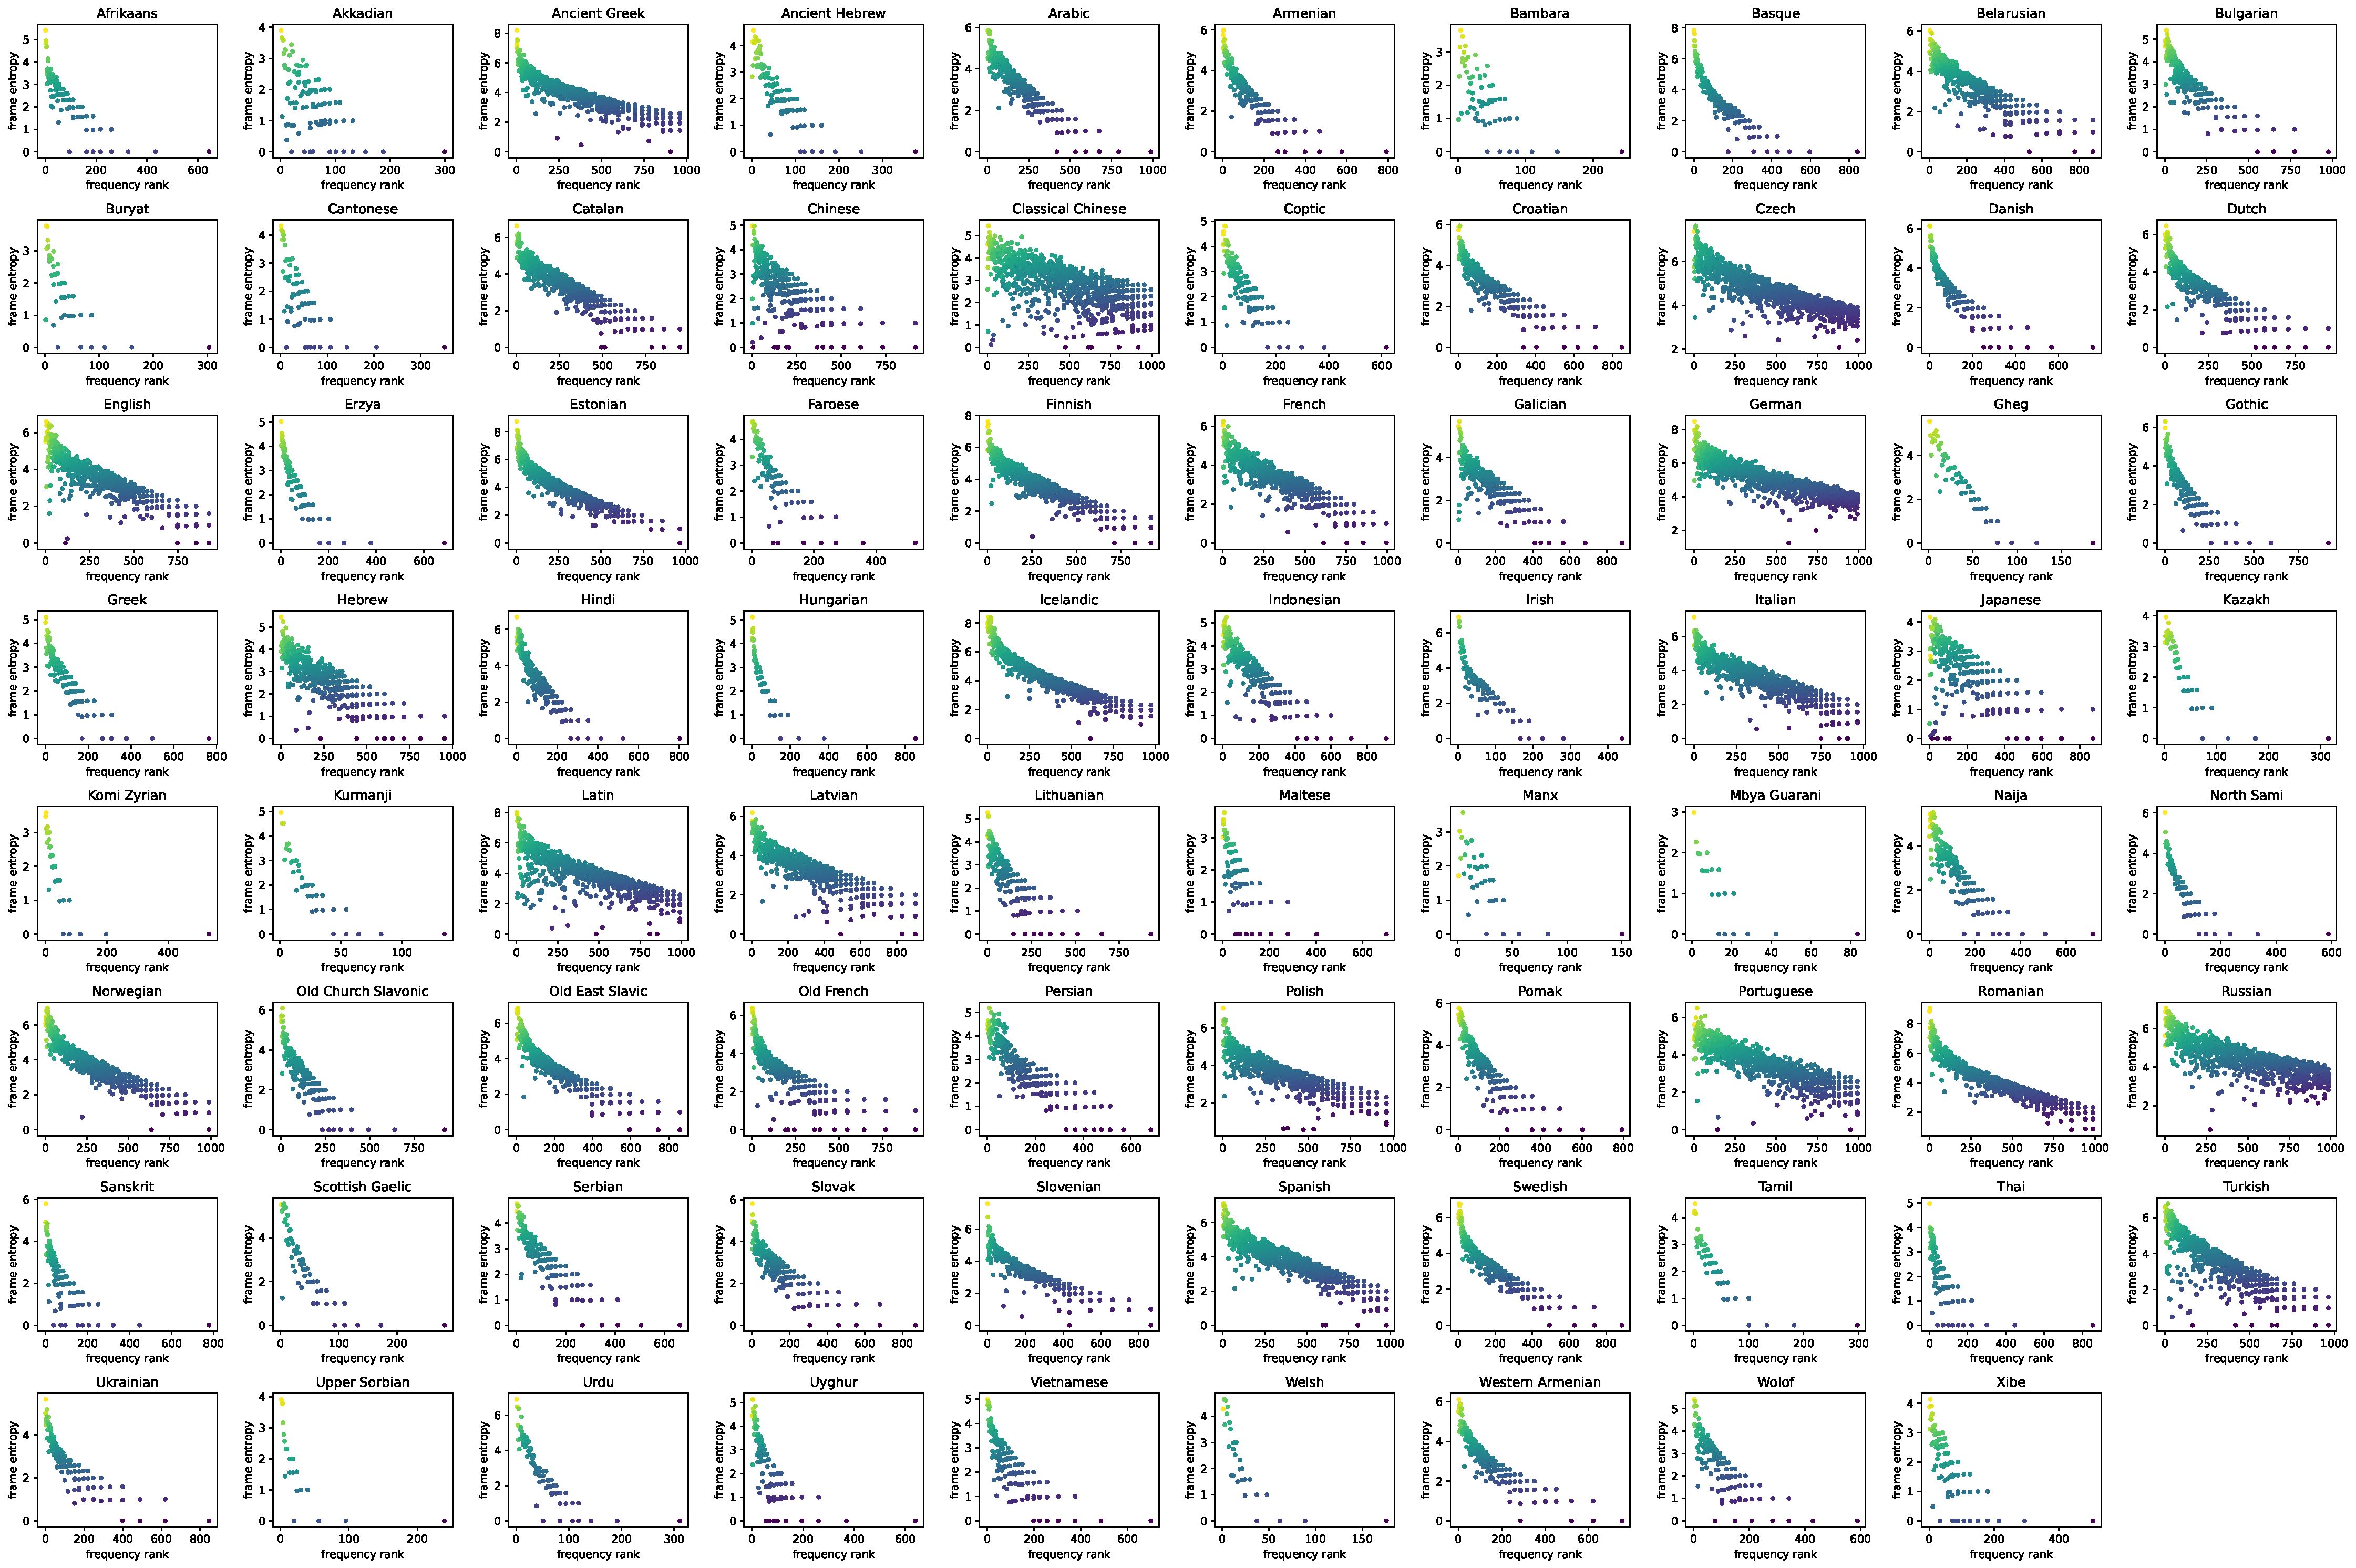
\includegraphics[width=\textwidth]{figures/joint_entropy_freq.pdf}
  \caption{Scatter plots showing relationship between valency frame entropy and frequency rank of verbs, color shows number of frames associated with the verb}
  \label{fig:joint_entropy_freq}
\end{sidewaysfigure}


% subsampling results

Results from subsampling are presented in xxx. As expected, the correlation strength decreased across the board, particularly for languages such as xxx. 

% subsampling discussion

The subsampling results highlights the need as a next step to analyze the results for the varying correlation. This could be because of language structure. Complexity vs the verbal system 

% correlation between frequency and dependency relation entropy

As an additional test, we also confirm that individual dependency relations do not correlate with frequency. This is as expected and confirms the validity of valency frame as a suitable level for analyzing argument structure.

% number of frames
number of frames should an even stronger correlation with frequency - of course. 


\section{Experiment 3: Word order or case? Cross-lingual variation in valency encoding strategies}\label{sec:exp3-ablation}
\subsection{Introduction}

Typological differences regarding word order and case marking necessarily means that different languages will have to use different strategies for encoding valency frames. On the one hand, it is a straightforward matter that a language cannot use case marking to encode a valency frame if it does not have case marking and a language with more flexible word order is less likely to use word order to encode its valency frame. On the other hand, the trade-off between word order and case marking in languages has been a well-studied topic in typology.

\subsection{Methodology}

% correlation strength comparison
For this experiment, we compare use only valency frame information  
- valency frame without word order information
- valency frame without case marking
- valency frame without word order and case marking information

% conditional entropy
- conditional entropy of word order information 
-  conditional entropy of word order information 
- calculate conditional entropy using the chain rule
a variation of
$$H(X_{k} | V = v, X_{1},\cdots,X_{n} \setminus X_{k}) = H( V = v, X_{1},\cdots,X_{n}) - H( V = v, X_{1},\cdots,X_{n}\setminus X_{k})$$

\subsection{Results and analysis}

% correlation strength comparison

Lower correlation strength are observed


% conditional entropy as percentage of the full entropy 
Delta between them 

\section{Experiment 4: Verb specificity and the argument-adjunct distinction}\label{sec:exp4-verb-specificity}

\subsection{Introduction}

Let us reexamine the argument-adjunct distinction in argument structure again. This distinction is relevant to syntax and semantics at a sentential level and usually formulated to state that the former is obligatory to complete the meaning of the verb, and the latter not. As it is concerned with morphosyntax first and foremost, this study focuses on the syntactic observation of \textit{verb specificity} \citep[cf.]{haspelmath2015a}, namely that verbs are more selective with regard to arguments but can be more freely used with adjuncts. 

% This experiment seeks to quantify the verb specificity by looking at the variance of dependency relation entropy when conditioned the verb. The entropy measures the average surprisal associated with this relation (including presence, word order and case marking) when given the verb. If a verb never or always appears with a certain dependency relation with a certain word order and case marking, the entropy of this dependency relation conditioned on the verb will be 0; the opposite scenario, where a verb is equally likely to appear with or without certain dependency frame, would result in the highest possible entropy. The specific ceiling value is dependent upon the possible `frames' of this entropy given the number of case marking and word order flexibility and will vary by language.

% Recall the bimodal distribution of transitive verbs observed \subsection{subsec:transitivity-lexicon}, verbs that are highly transitive or highly intransitive will have high entropy, carrier more information. Verb specific feature leads to higher entropy.


% The less verb specific a dependency is, the more uniform it will be between verbs resulting in lower entropy in general. This is on an entropy per dependency relation level.

\subsection{Methodology}

$$H(X_{k} | V = v, X_{1},\cdots,X_{n} \setminus X_{k}) = H( V = v, X_{1},\cdots,X_{n}) - H( V = v, X_{1},\cdots,X_{n}\setminus X_{k})$$

\subsection{Results and analysis}

\section{Experiment 5: Frequency correlation with verb entropy}\label{sec:exp5-verb-entropy}

\subsection{Introduction}

So far the experiments have focused on calculating the valency frame entropy conditioned on verb choice. While this does not necessitate the lexeme-based view of valency, lexeme is still the level at which experiments are performed and analysis made. As the hypotheses themselves are motivated by constraints on language structure that derive from its communicative function, they should nevertheless be neutral with respect to which theory of valency one subscribes to. 

Consequently, if one were to adopt the frame-based view of valency and insist on using the frame as the level of analysis, a symmetric hypothesis can be made: namely that given a new metric of verb entropy conditioned on valency frame, we would see a similar frequency effect where the entropy of lexical choice would correlate with the frequency of the valency frame. 

This experiment undertakes to examine exactly that hypothesis and verify the expected symmetry.

\subsection{Methodology}

The entropy value for the verb given a single slot is

$$
H(V|X_{k}=x)=
-\sum\limits_{v\in{}\mathcal{V}}{P(v|X_k=x)\log_{2}{P(v|X_k=x)}}
$$

extend it to multiple argument slots, we have

$$
H(V|X_1=x_1,\ldots,X_n=x_n)=
-\sum\limits_{v\in{}\mathcal{V}}{P(v|X_1=x_1,\ldots,X_n=x_n)\log_2P(v|X_1=x_1,\ldots,X_n=x_n)}
$$

\subsection{Results and analysis}

